%%%%%%%%%%%%%%%%%%%%%%%%%%%%%%%%%%%%%%%%%%%%%%%%%%%%%%%%%%%%%%%%%%%
%
% First comes an example EPS file -- just ignore it and
% proceed on the \documentclass line
% your LaTeX will extract the file if required
%
\RequirePackage{fix-cm}
%
%\documentclass{svjour3}                     % onecolumn (standard format)
%\documentclass[smallcondensed]{svjour3}     % onecolumn (ditto)
\documentclass[smallextended]{svjour3}       % onecolumn (second format)
%\documentclass[twocolumn]{svjour3}          % twocolumn
%
\smartqed  % flush right qed marks, e.g. at end of proof
%
\usepackage{graphicx}
%
% \usepackage{mathptmx}      % use Times fonts if available on your TeX system
%
% insert here the call for the packages your document requires
%\usepackage{latexsym}
\usepackage{amsmath}
\usepackage{amssymb}
\usepackage{scalefnt}
\usepackage{graphicx}
\usepackage{hyperref}
\usepackage{subfigure}
\usepackage{enumerate}
\usepackage{caption}
\usepackage{booktabs}
\usepackage{natbib} 
\usepackage{lipsum}  
\usepackage{xfrac}
\usepackage{indentfirst}
\usepackage[brazil]{babel}
\hyphenation{re-gis-tra-dos}


\usepackage{color}
\usepackage[normalem]{ulem}
\definecolor{darkgreen}{RGB}{0,80,0}
\newcommand{\old}[1]{{\color{red}\sout{#1}}}
\newcommand{\new}[1]{{\color{blue}#1}}
\newcommand{\comment}[1]{{\color{darkgreen}{\bfseries [#1]}}}

% etc.
%
% please place your own definitions here and don't use \def but
% \newcommand{}{}
%
% Insert the name of "your journal" with
% \journalname{myjournal}
%
\begin{document}

\title{Técnica $\sfrac{H}{V}$ para determinação da elipticidade da onda Rayleigh}
\subtitle{}

%\titlerunning{Dielectric permittivity effects in the detection of tree roots using GPR}        % if too long for running head

\author{Danilo Portela de Oliveira¹\and Marcelo Peres Rocha¹         
}

%\authorrunning{Short form of author list} % if too long for running head

\institute{Danilo Portela de Oliveira \at
              Campus Universitário Darcy Ribeiro - Universidade de Brasília - UnB, Asa Norte. %Prédio SG 13. \\
              %Tel.: +55 61 99287-5004\\
              %Fax: +123-45-678910
              \\
              \email{daniloportela97@gmail.com}           %  \\
%             \emph{Present address:} of F. Author  %  if needed
           %\and
           %Luísa Lins \at
             % Campus Universitário Darcy Ribeiro - Universidade de Brasília - UnB, Asa Norte. Prédio SG 13.
}

\date{¹Universidade de Brasília, UnB, Brasil}
% The correct dates will be entered by the editor


\maketitle

% -----------------------------------------------

\begin{abstract}

% \lipsum[1]

Muitas técnicas geofísicas podem ser utilizadas para obter o perfil de velocidade da onda de cisalhamento para aplicação próxima à superfície. Porém, mais recentemente vem sendo utilizada uma técnica em que é realizada uma inversão conjunta da curva da razão espectral H/V e da curva de dispersão extraída a partir da análise multicanal das ondas de superfície (MASW). Contudo, em alguns casos, para obter a curva de dispersão na faixa de frequência para aplicação na engenharia (1 a 30 Hz) torna-se mais difícil. Nesse caso, a curva de dispersão pode ser indiretamente invertida de todos os pontos disponíveis da curva de frequência da onda Rayleigh para velocidade e profundidade da onda de cisalhamento. Como resultado, temos uma série de valores (velocidade e profundidade da onda s) através dos quais uma tendência de melhor ajuste pode ser passado. O melhor ajuste nos dá uma ideia da taxa de aumento da velocidade da onda de cisalhamento com a profundidade e a velocidade da onda de cisalhamento a um metro de profundidade. Com essa informação, podemos posteriormente utilizar para inverter a curva de elipticidade da onda de Rayleigh.  

\keywords{Sismologia \and Ondas Rayleigh \and Arranjos sísmicos \and Razão $\sfrac{H}{V}$
}
% \PACS{PACS code1 \and PACS code2 \and more}
% \subclass{MSC code1 \and MSC code2 \and more}
\end{abstract}

% -----------------------------------------------

\newpage

\section{Introdução}

A relação de ruído espectral horizontal para vertical (relação H/V) \citep{nakamura1989method} tem sido frequentemente usada para estudar a amplificação do local e a estrutura da crosta rasa e tem sido particularmente útil na avaliação de risco sísmico (por exemplo, \citealp{field1993theoretical}; \citealp{bonilla1997site}; \citealp{konno1998ground}; \citealp{riepl1998detailed}; \citealp{parolai2002new}; \citealp{bonnefoy2006nature}). No entanto, a relação H/V pode ser influenciada pela composição do campo de ondas de ruído (ou seja, Rayleigh, Love e ondas de corpo; consulte \citealp{bonnefoy2006nature} para uma revisão e \citealp{koper2010composition} para uma pesquisa global), dificultando a interpretação da relação H/V. A relação entre a elipticidade da onda Rayleigh (ou razão H/V da onda Rayleigh) com a estrutura rasa 1-D da Terra, por outro lado, está bem definida \citep{tanimoto2008zh}. 

A extração da elipticidade da onda de Rayleigh usando técnicas de matriz de 3 componentes tem se mostrado bastante confiável \citep{poggi2010estimating}. Recentemente, técnicas multicomponentes de correlação cruzada de ruído ambiental também foram desenvolvidas para obter medições robustas da relação de amplitude H/V da onda Rayleigh (\citealp{lin2014upper}; \citealp{lin20143}). Esta técnica mais recente usa correlações cruzadas de ruído entre pares de estações para aproximar as funções de Green da onda Rayleigh entre um par de estações onde uma estação é considerada uma fonte virtual e a outra estação é considerada um receptor. As correlações cruzadas podem então ser usadas para fazer observações da relação H/V da onda Rayleigh empregando uma força vertical ou radial na fonte virtual e medindo a relação de amplitude entre os componentes radial e vertical no receptor.

Embora a correlação cruzada de ruído tenha a vantagem de isolar as ondas de Rayleigh do ruído ambiental, a interpretação do resultado pode ser difícil se o campo de ruído não for semidifusivo. 
A aproximação de campo distante ajuda a garantir um campo de ruído semidifusivo, mas as estações de origem virtual devem estar a pelo menos três comprimentos de onda de distância das estações de destino. A incerteza da medição também pode ser alta se não houver estações suficientes atuando como fontes virtuais.

Então, este texto objetiva por meio de uma revisão bibliográfica (do artigo \citealp{ullah2016thickness}) exibir estudos utilizando este método em um local quase pantanoso, localizado em Colônia, na cidade de São Paulo, Brasil, para a estimativa da espessura do pacote de sedimentos não consolidados sobre o leito rochoso (embasamento neste caso). 

A técnica H/V é empregada no sítio em Colônia por causa de sua configuração geológica, pois possui um pacote espesso de sedimentos não consolidados sobrepostos a rochas duras do embasamento, essa interface não consolidada do solo rochoso dá origem a uma velocidade muito alta e contraste de densidade que é muito favorável para aplicação \textit{horizontal-over-vertical} (H/V).

% -----------------------------------------------

\section{Geologia do local}

A estrutura da Colônia está localizada na periferia sul da cidade de São Paulo, Brasil (Fig. \ref{geologia}). Tem uma geometria circular (diâmetro de 3,6 km) compreendendo um anel anular de colinas que circundam uma depressão. A estrutura é majoritariamente um pântano. Sua origem é atribuída a um impacto de meteorito \citep{riccomini1989colonia}. A estrutura é formada em rochas do embasamento cristalino de idade neoproterozóica e a depressão é preenchida principalmente por sedimentos ricos em matéria orgânica de idade quaternária. Os principais tipos rochosos do embasamento compreendem xisto, quartzito, gnaisse, migmatito, diorito, quartzo-diorito \citep{sadowski1974tectonica}.

A profundidade total, estimada por investigação de reflexão sísmica (Fig. \ref{geologia}), que não atingiu a parte central da estrutura \citep{riccomini2011colonia} é de cerca de 340 m (preenchimento sedimentar mais brecha). A função de velocidade de empilhamento nesta investigação (Fig. \ref{fun_vel}) mostrou um incremento contínuo da velocidade da onda P com a profundidade, começando de aproximadamente 1500 m/s para 2150 m/s, o que é consistente com o aumento esperado da compactação dos sedimentos.

\begin{figure}[!hbtp]
  \begin{center}
  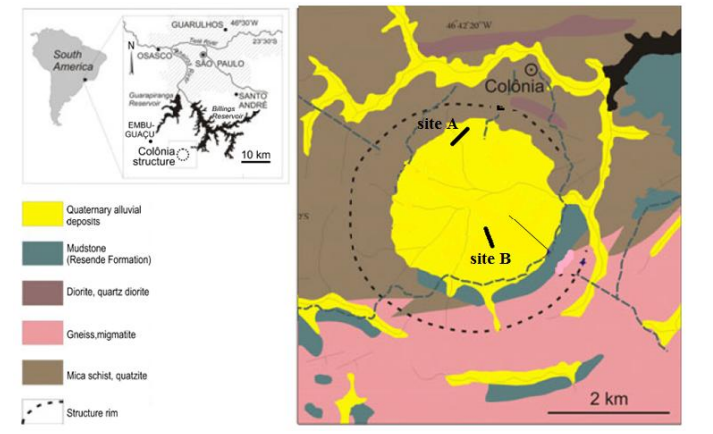
\includegraphics[scale=0.8]{Figures/fig1.png}
  \end{center}
  \caption{Localização (esquerda) e mapa geológico da estrutura da Colônia. As linhas grossas pretas indicam os locais dos testes MASW, enquanto as linhas finas indicam a linha de reflexão. (Modificado de \citealp{riccomini2011colonia}).
  }
  \label{geologia}
\end{figure}

\begin{figure}[!hbtp]
  \begin{center}
  
  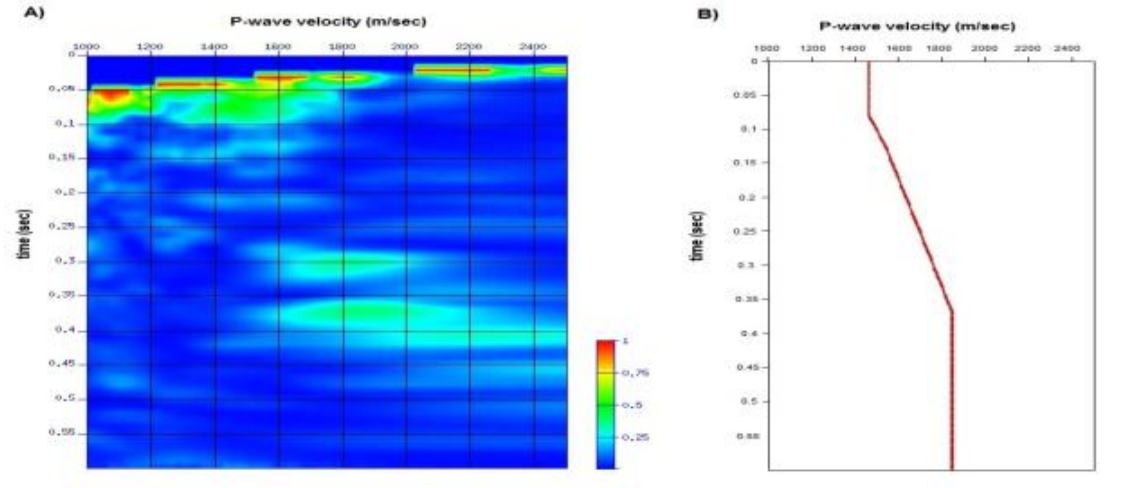
\includegraphics[scale=0.5]{Figures/fig2.png}
  \end{center}
  \caption{Figura com painel (A) e (B), onde a função de velocidade de empilhamento cdp é adquirido a 750 ms da investigação de reflexão sísmica de Colônia (onda P) (modificado de \citealp{riccomini2011colonia}).
  }
  \label{fun_vel}
\end{figure}

% -----------------------------------------------

\section{Metodologia}
\label{methods}

\subsection{Ondas Rayleigh}

As ondas Rayleigh são ondas de superfície que movimentam as partículas do meio de maneira polarizada ao longo de uma elipse vertical em sentido oposto ao da propagação (retrogrado). A razão entre as dimensões dos eixos horizontal e vertical da elipse de movimento de partícula define a elipticidade da onda Rayleigh, que é, sobre certas circunstâncias, dependente da estrutura local abaixo das estações \citep{berbellini2019constraining}.

\begin{figure}[!hbtp]
\begin{center}

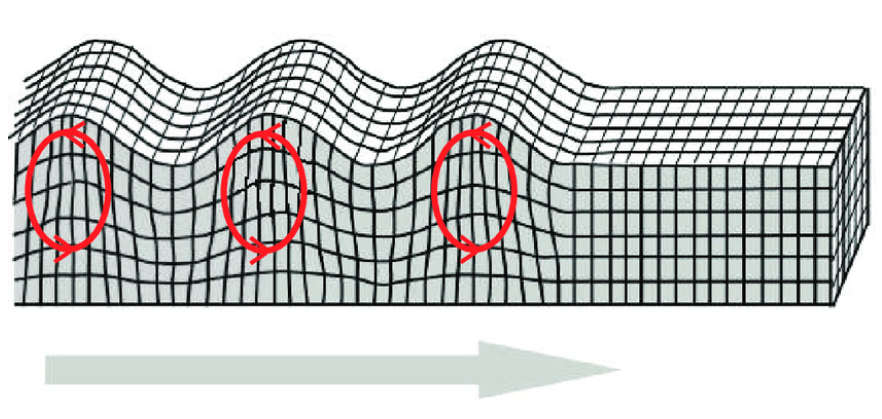
\includegraphics[scale=0.5]{Figures/ondas_rayleigh.png}
\end{center}
\caption{Comportamento das ondas Rayleigh na superfície terrestre \citep{de2009filtragem}.}
\label{ondas_rayleigh}
\end{figure}

\subsection{Elipticidade das Ondas Rayleigh}

Essa técnica, também chamada de Razão H/V da onda Rayleigh \citep{workman2017determination}, pode ser utilizada tanto para uma única estação, quanto para um arranjo de estações. A desvantagem conceitual da aplicação desse método para uma única estação é que, apesar de ser possível obter a elipse de movimento das partículas, não conseguem resolver a ambiguidade de 180 graus relacionada com a determinação do azimute reverso (backazimuth), não sendo possível identificar se o movimento é retrogrado ou não, e consequentemente, a direção de chegada das ondas Rayleigh (\citealp{workman2017determination}, \citealp{berbellini2019constraining}).

\subsection{inversão}

A partir de medidas do espectro H/V para diferentes períodos, é construída a curva de elipticidade média para as estações pertencentes ao arranjo. A curva de elipticidade é invertida para obtenção do modelo 1D de velocidade da onda S em relação à profundidade, logo abaixo do arranjo das estações (no centro do arranjo). Esse modelo pode ser interpretado em termos das descontinuidades existentes sob o arranjo das estações.

Para a inversão da elipticidade e para amostrar o espaço de parâmetros, utilizou-se o \textit{eighborhood algorithm} (NA) \citep{wathelet2008array} que é um método livre de derivadas em comparação com o método linearizado \citep{menke1989geophysical}. Este método (NA) auto-adaptativo amostra o espaço do modelo para encontrar um conjunto de modelos que melhor se ajusta aos dados reais. Para cada modelo amostrado, o algoritmo de inversão compara dados previstos com dados reais (usando a abordagem de modo normal de \cite{herrmann2013computer} para calcular curvas de elipticidade e avaliar uma função de custo). 

Dessa forma, o cálculo da função de custo leva em consideração o desajuste entre os dados reais e os valores previstos e geralmente também contém um termo para regularizar as soluções. Um termo de regularização é necessário quando a parametrização é feita de muitas camadas finas para promover os modelos mais suaves. A função custo é definida como:

\begin{equation}\label{eq:cost_function}
  c = \sum_{i=1}^{N_m} \frac{[d_{obs}^i - g^i(m)]^2}{(\sigma^i_{D})^2} + A \cdot N_m \sum_{j=1}^{N_L} [v_s^{j - 1} - 2v_s^{j} + v_s^{j + 1}]^2 
\end{equation}

Onde $d_{obs}^i$ são os dados observados, $g^i(m)$ são valores teóricos de elipticidade calculados usando um formalismo de modo normal para o modelo amostrado $m$, $\sigma^i_{D}$ é a variância da medição, $N_m$ é o número de medições, $N_L$ é o número de camadas, $A$ é um fator de escala e $v_s$ é a velocidade da onda de cisalhamento. 

O primeiro termo é o desajuste entre os dados observados e previstos, o segundo é o termo de regularização. $A$ é um fator de escala determinado por tentativa e erro: se $A$ for muito pequeno, os dados observados serão superajustados, enquanto o modelo resultante mostrará descontinuidades muito irrealistas. Por outro lado, se $A$ for muito grande, o modelo será plano e os dados observados não serão bem ajustados. Um bom fator $A$ produz modelos realistas enquanto ajusta bem os dados observados. 

% -----------------------------------------------

\section{Resultados}
\label{results}

As técnicas de curva H/V são fortemente condicionadas pelas propriedades (isto é, contraste de profundidade e impedância) da interface entre o sedimento não consolidado e o leito rochoso \citep{parolai2005joint}, embora sejam pouco informativas sobre a velocidade da onda s das camadas sedimentares. Por outro lado, as curvas de dispersão provenientes da técnica de matriz (ou seja, MASW, análise multicanal de ondas de superfície \citealp{park1999multichannel}) restringem principalmente a estrutura de velocidade da onda s do solo subterrâneo. Porém, a curva de dispersão fornece informações incertas sobre a subsuperfície mais profunda, especialmente abaixo da frequência fundamental do local devido ao efeito de filtragem da média; portanto, quando H/V ou curvas de dispersão são usadas individualmente para a recuperação da estrutura da subsuperfície, há um \textit{trade-off} solucionável entre os parâmetros do modelo (velocidade e espessura das camadas do solo) que dificulta os resultados da análise de inversão.

Além disso, adquirir MASW e gravação de ruído ambiental no mesmo local pode não ser possível devido a alguns problemas locais em configurações de campo, como acessibilidade, como na estrutura da Colônia, onde a maior parte da estrutura é coberta por vegetação densa e água, dificultando na gravação do MASW e ruído ambiental nos mesmos locais, para mapear a estimativa da espessura do pacote de sedimentos. Dessa forma, abordaram que a tendência média de aumento da velocidade da onda de cisalhamento com a profundidade pode ser obtida a partir da inversão direta da curva de dispersão, ou seja, a abordagem foi que em qualquer local acessível da estrutura uma curva de dispersão experimental pode ser obtida através do MASW (Fig. \ref{geologia}). 

Para a estimativa da curva H/V, precisaram do registro do ruído ambiental em três componentes (dois horizontais e um vertical) que obtiveram a partir de 7 medições do ruído ambiental em 6 locais diferentes mostrados na (Fig. \ref{stations}) com um sismômetro de 3 componentes de banda larga \textit{Nanometrics Trillium} compacto de 120 s. Realizaram a gravação do ruído ambiental por 5 horas em cinco locais, enquanto que nas estações CLN4 e CLN5 a gravação foi de 24 horas (Fig. \ref{stations}). A gravação foi aumentada para evitar ruído cultural, pois havia atividade agrícola próxima.

A gravação do ruído ambiental foi feita seguindo as diretrizes desenvolvidas nas recomendações do \cite{acerra2004guidelines}. Para obter a frequência fundamental do local, foi processada uma janela de gravação de uma hora e seguiu-se a condição de confiabilidade proposta pelo \cite{acerra2004guidelines} para a curva H/V e pico, (Fig. \ref{hv_curva}) indica as curvas H/V de todas as estações. A curva de dispersão recuperada do MASW analisando todos os dados (Fig. \ref{curva_disp}) é obtida apenas em uma banda de frequência estreita (1.1 - 3.8 Hz) Fig. \ref{curva_disp}d. O levantamento MASW desses dois locais diferentes A e B (Fig. \ref{geologia}) são analisados, a imagem de dispersão das matrizes MASW é fornecida na Fig. \ref{curva_disp}a, b, c. Em A, os dados da fonte ativa não fornecem uma imagem de dispersão clara, por isso são omitidos da análise. A curva de dispersão exponencial obtida a partir dos dados é ampliada (para uma visibilidade clara na escala vertical) (Fig. \ref{curva_disp}d).


\begin{table}[!hbtp]
\caption{Parâmetros de aquisição MASW para fonte ativa e passiva.}
\label{table_parameters}
\centering
\begin{tabular}{@{}lccc@{}}
\toprule
Tipo de MASW         & Ativo & Passivo &  \\ \midrule
Fonte & Marreta 10 Kg         & Ruído cultural                    \\
Deslocamento mínimo (m)   & 1, 5, 6       &                         \\
Intervalo entre Geofones (m)      & 1             & 1                             \\
Número de geofones             & 96              & 96                                    \\ 
Tamanho do arranjo               & 95              & 95                                   \\ 
Intervalo de amostragem (ms)              & 0.5              &                                      \\ 
Duração do(s) registro(s)              & 1              & 15, 20, 30                                  \\ \bottomrule
\end{tabular}
\end{table}

\begin{figure}[!hbtp]
  \begin{center}
  
  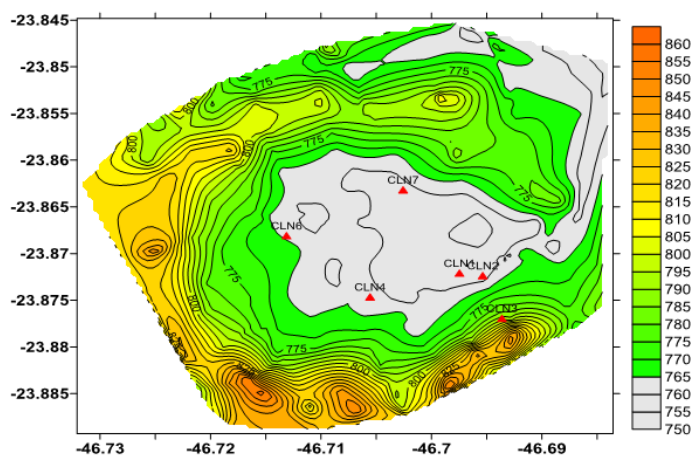
\includegraphics[scale=0.7]{Figures/fig3.png}
  \end{center}
  \caption{Mapa de contorno topográfico (intervalo de contorno 5m) da estrutura de Colônia. Os triângulos indicam a localização das estações usadas para gravação de ruído ambiental. CLN4 e CLN5 estão no mesmo local, por isso é mostrado apenas CLN4. (A barra de legenda à direita mostra a escala dos contornos em m).}
  \label{stations}
\end{figure}

\begin{figure}[!hbtp]
  \begin{center}
  
  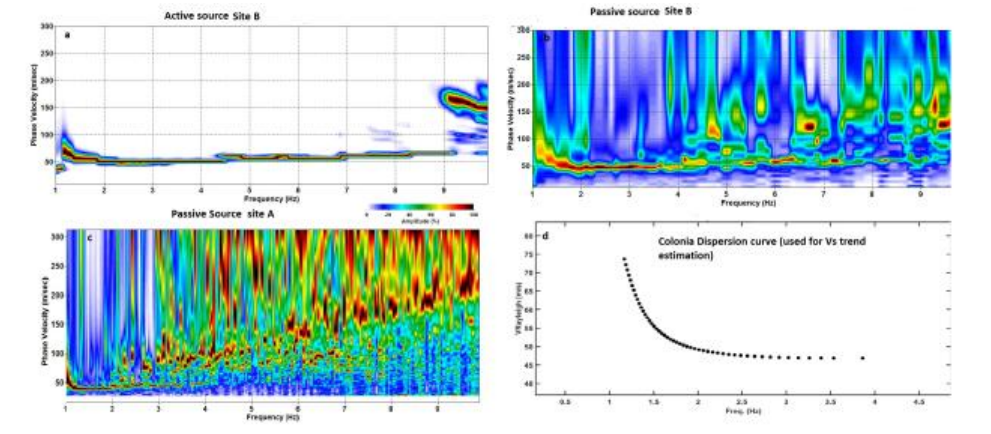
\includegraphics[scale=0.6]{Figures/fig4.png}
  \end{center}
  \caption{Mostra as imagens da curva de dispersão dos registros experimentais do local B (a velocidade nas imagens da curva de dispersão é em m/s). (b) Fonte passiva das imagens da curva de dispersão no local B (c). Imagens da curva de dispersão da fonte passiva do local (d). A curva de dispersão experimental obtida dos dados em Colônia é mostrada na parte inferior (usada para estimativa de tendência vs).}
  \label{curva_disp}
\end{figure}

\begin{figure}[!hbtp]
  \begin{center}
  
  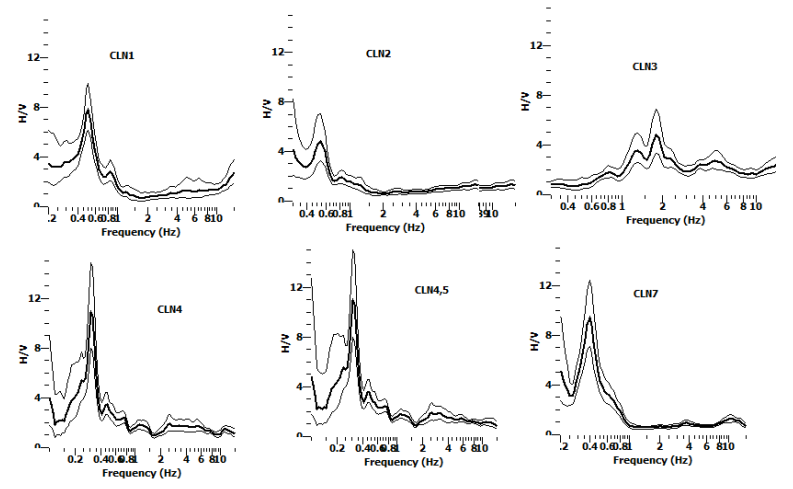
\includegraphics[scale=0.75]{Figures/fig5.png}
  \end{center}
  \caption{Curvas H/V de todas as estações. Todas as curvas são obtidas cumprindo os critérios para curva clara e pico, a linha em negrito é a curva H/V, as linhas estreitas inferior e superior indicam o limite superior e inferior do desvio padrão.}
  \label{hv_curva}
\end{figure}
\newpage

\subsection{Inversão para recuperação da velocidade da onda de cisalhamento}

Para realizar a inversão da elipticidade, utilizou-se o algoritmo de vizinhança (NA) \citep{wathelet2008array} que é um método livre de derivadas em comparação com o método linearizado \citep{menke1989geophysical}. NA pertence à família de estratégias de inversão de otimização global, como algoritmo genético. \cite{sambridge2002monte} reviu em detalhes o aspecto teórico e a aplicação dessa abordagem de inversão. A NA é considerada uma estratégia de inversão melhor porque tem vantagem sobre as outras abordagens, pois utiliza todas as informações do modelo anterior para amostrar o novo modelo \citep{sambridge1999geophysical}. O desajuste é estimado usando a eq.(~\ref{eq:desajuste})  

\begin{equation}\label{eq:desajuste}
  misfit_{Ellipticity} = \sqrt{\frac{1}{N} \sum_{i=1}^{N}\left(\frac{log(Emod) - log(Exp)}{\sigma_i^2}\right)^2} 
\end{equation}

Onde $Exp$ é uma curva de elipticidade experimental na frequência $f$, $Emod$ é a curva de elipticidade modelada na frequência $f$, $\sigma_i$ são os erros de medição associados e $N$ é o número da amostra de frequência.

A curva H/V é considerada como a curva de elipse da onda Rayleigh, que é empregada em quase todos os algoritmos de inversão de curva H/V, porém a curva H/V não é a verdadeira representação da elipticidade da onda Rayleigh, pois ambas as ondas Rayleigh e Love contribuem para o espectro H/V \citep{bonnefoy2006h} e a presença de ambos os tipos de onda de superfície devem ser considerados para algoritmos de inversão. 

Portanto, a proporção entre as ondas Rayleigh e Love no campo de ondas de ruído deve ser inferida ou assumida antes da inversão. Para solucionar esse problema e minimizar a contribuição da onda Love para o componente horizontal da curva H/V, \cite{hobiger2009single} propôs uma técnica conhecida como RayDec para a estimativa da elipticidade da onda Rayleigh a partir de um único sensor de três componentes, utilizando a componente vertical como um gatilho mestre e empilhando um grande número de componentes horizontais. (ver detalhes \citealp{hobiger2009single}). 

Utilizaram o RayDec para obter a curva de elipticidade para cada local de registro do ruído ambiental. O flanco direito da elipticidade é usado para análise de inversão \citep{hobiger2013ground}. No entanto, o flanco esquerdo é considerado  para colocar restrições na frequência de pico da curva de elipticidade (H/V). Usaram 30\% do comprimento da frequência de pico no flanco esquerdo e o dobro da frequência de pico no flanco direito. A parte restante da curva de elipticidade não é considerada para inversões. A tendência de aumento da velocidade da onda de cisalhamento e a espessura do pacote sedimentar (h) são entradas para a inversão da curva de elipticidade e os perfis de inversão são obtidos. (Fig. \ref{elipticidade}).

\begin{figure}[!hbtp]
  \begin{center}
  
  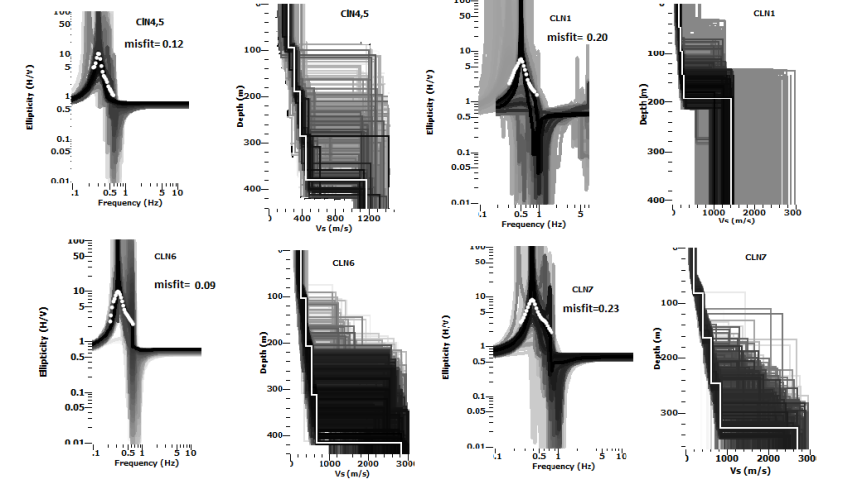
\includegraphics[scale=0.7]{Figures/fig7.png}
  \end{center}
  \caption{Perfis de inversão e valores desajustados para CLN4,5, CLN1, CLN6 e CLN7. O perfil do modelo desajustado mais baixo do VS é mostrado em branco para todas as estações.}
  \label{elipticidade}
\end{figure}
\newpage

% -----------------------------------------------

\section{Discussões e Conclusões}

O resultado obtido para as curvas H/V segue a tendência do ambiente geológico local (Colônia). Temos que as estações CLN4,5 e 6 mostraram a mesma frequência de ressonância fundamental que, com base nesse tipo de abordagem de interpretação, nos dá a espessura do solo não consolidado em torno de 400 m. \cite{riccomini2011colonia} mostra que a espessura do sedimento não consolidado encontra-se em torno de 340 m usando sísmica de reflexão, mas quase na mesma posição periférica da estrutura circular de Colônia. A espessura do sedimento em direção à borda da estrutura em forma de ``tigela" diminui, o que é identificável a partir da estação CLN3, que mostrou uma espessura de 15 metros. Como discutido anteriormente, uma inversão de elipticidade sozinha produz resultados ambíguos. Então, se forem adicionadas informações que restringem a estrutura da onda de cisalhamento superficial, a inversão de elipticidade pode então ser usada para restringir a parte mais profunda da estrutura. Contudo, no caso de leito rochoso muito profundo, a curva de dispersão experimental obtida mostra apenas uma parte de toda a curva de dispersão e não a curva completa devido ao ambiente geológico local. Para restringir a velocidade da onda de cisalhamento superficial nessas situações, pode-se adicionar à inversão descobrindo a tendência do aumento da velocidade da onda de cisalhamento com a profundidade a partir da utilização dessa curva de dispersão experimental de banda de frequência estreita pelo melhor ajuste dos valores de profundidade $V_s$. O que fornece informações sobre a tendência de aumento da velocidade a um metro de profundidade. A frequência fundamental junto com a tendência de aumento da onda s e a velocidade da onda s a um metro de profundidade são usadas para encontrar a espessura composta (h) do pacote de sedimentos. Todas essas informações podem ser fornecidas para a inversão da curva de elipticidade no final para obter o perfil 1D da velocidade da onda de cisalhamento.

Portanto, utilizaremos essa técnica no projeto de pesquisa do mestrado com o objetivo de estudar a estrutura crustal sob a região da Província Mineral de Carajás e áreas adjacentes. Esperamos alcançar níveis de resolução suficientes para definir as interfaces entre a crosta e o manto (Moho), e eventualmente entre a litosfera e a astenosfera (LAB). Esperamos também que outras descontinuidades possam ser identificadas, como a entre a crosta superior e inferior (Conrad), ou outras mais rasas. 

\newpage

% -----------------------------------------------


%\begin{acknowledgements}
%We would like to thank Dr. Welitom Rodrigues Borges for the assistance with data processing and for providing the antenna used in this research.  
%\end{acknowledgements}

%\clearpage
\bibliographystyle{seg}  % style file is seg.bst
\bibliography{References}

\end{document}

% -----------------------------------------------
